
\chapter{Introduction}
\label{chap:Introduction} 

\section{Molecular Biology}
\label{sec:MolecularBiology}

Molecular biology is the study of the molecular basis of biology.
It is mostly concerned with the understanding of the systems and processes
that occur within a living cell.
Naturally, the field overlaps considerably with other areas, 
such as genetics (the study of genes and heredity) and biochemistry (the study
of the chemical processes of life).

While the field itself is rather broad, much of it is underpinned by what is
referred to as the central dogma of molecular biology -- 
DNA makes RNA makes proteins.
This central dogma describes the flow of information within a cell and the
processes and control mechanisms which regulate this process.
Naturally, many of these processes are highly complicated and poorly
understood, but much progress has been made since the discovery of DNA in the
1950s to understand these processes.
Figure~\ref{fig:processes} shows the most important of these processes and how
they convert between the three most important classes of molecules in the cell.

\begin{figure}
  \centering
  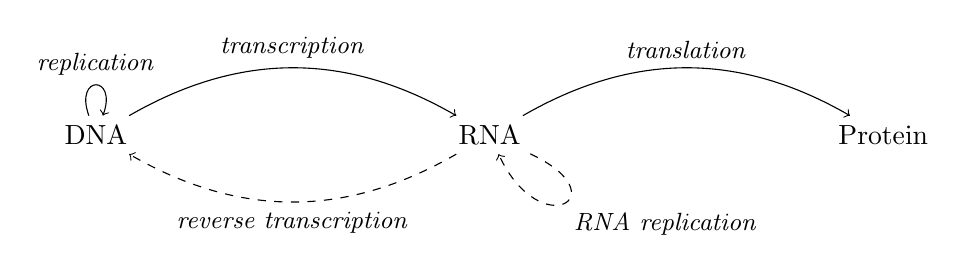
\begin{tikzpicture}[node distance=5cm, auto]
    \node (D) {DNA};
    \node (R) [right of=D] {RNA};
    \node (P) [right of=R] {Protein};
    \draw[->, bend left] (D) to node {\small \textit{transcription}} (R);
    \draw[->, bend left] (R) to node {\small \textit{translation}} (P);
    \draw[->] (D) to [out=110,in=70,looseness=8] 
                node {\small\textit{replication}} (D);

    \draw[->, dashed, bend left] 
      (R) to node {\small \textit{reverse transcription}} (D);
    \draw[->, dashed] (R) to [out=335,in=295,looseness=8] 
                node {\small\textit{RNA replication}} (R);
  \end{tikzpicture}
  \caption{The main processes in molecular biology. The three most common are
    shown using solid lines while two important but less common processes are
    shown in dotted lines.
    \label{fig:processes}}
\end{figure}

Molecules of DNA are the cell's long term storage mechanism -- recent research
estimates the half-life of DNA to be 521 years\cite{DNAhalflife}.
DNA molecules are long sequences of simple nucleotides which encode all the
genetic information of the cell.
Each nucleotide contains a nucleobase which is either Adenine, Guanine,
Thymine or Cytosine (A,G,T or C) and it is the sequence of so called bases which
determines the information content of the molecule.
DNA is double-stranded -- each base in the chain forms a hydrogen bond with a
base from a complementary chain of DNA.
These strands are coiled around each other into DNA's characteristic 
double-helix structure.

The data stored in DNA is read by a molecule called RNA polymerase which 
produces an RNA copy of a section of the DNA in a process called
\textit{transcription}.
RNA is similar to DNA, but is short-lived (lasting minutes to hours) and so the
RNA copy is referred to as a messenger-RNA (mRNA) molecule.
This message is then read by a ribosome, a molecule which translates the mRNA 
into a protein, a process referred to as \textit{translation}.
Proteins a chain of amino acids which fold into a very specific shape and 
perform many important functions within the cell.
The region of DNA which encodes a particular protein is called a \textit{gene}.

The processes of transcription and translation through which genes are 
expressed (produce proteins) are typically very tightly
controlled by the cell, as this is the main way of influencing the levels of
various proteins within the cell and thus the cell's overall activity.

\subsection{Transcription}
\label{sec:transcription}

Both DNA and RNA have an alphabet of four symbols and so during transcription,
DNA's alphabet, $\{A,C,G,T\}$, is mapped one-to-one to that
of RNA, $\{A,C,G,U\}$, where thymine is replaced with uracil.
Transcription is clearly bijective, and indeed a less common process called
reverse-transcription performs the inverse mapping from RNA to DNA.

Transcription does not act on an entire DNA strand at once but instead
transcribes a small region of the DNA called a transcription unit, which
contains one or many genes.
These units are marked by promoters which are regions of DNA upstream
of the transcription unit that initiate transcription by causing RNA polymerase
to bind.
Control is commonly achieved by modulating promoter activity.


%Proteins are a sequence of amino acids, where each acid comes from an alphabet
%of 20 amino acids.
%Each acid is coded for by 3 base pairs of RNA, which are referred to
%collectively as a codon.
%Since there are $4^3$ possible codons and only 20 amino acids, the code is
%over complete -- several different codons map to the same amino acid.
%As well as coding for amino acids, three special codons (UAG, UAA and UGA) are
%known as stop codons as they terminate the translation of the protein.
%
%
%
%Ribosomes bind to the mRNA, reading the gene and creating the appropriate
%protein before detaching from the mRNA.
%mRNA is more fragile than DNA but is also targeted by exonucleases, a class of
%enzyme which degrade RNA molecules, preventing the production of more protein.
%Similar processes exist to degrade proteins over time, recycling their amino
%acids to form new proteins.
%These degradation processes mean that a gene must continue to be transcribed at
%a constant rate for the concentration of its protein to remain constant.
%


\section{Synthetic Biology}
\label{sec:synbio}

Synthetic biology is a relatively new
engineering discipline with the goal of applying standard engineering techniques
such as standardisation, characterisation and encapsulation of function to 
biology.
Synbio aims to use these design principles to combine existing phenomena to 
build new, artificial forms of life.
The field is often confused with its spiritual predecessor, genetic 
engineering, which although similar in some respects does not design new
organisms, but tinkers with existing ones without trying to understand the
underlying principals.

Synbio is often referred to as programming, but with DNA instead of computer
code.
An example project which captures this idea is Tabor's bacterial edge
detector\cite{edgeDetector}.
Bacteria were programmed to produce a colourless chemical messenger in the 
absence of light and to produce a dark pigment in the presence of light and the
chemical messenger.
When a film of these bacteria is exposed to a pattern of light and dark, the
messenger diffuses out from the dark regions and into the light, where it
stimulates the production of the pigment, leading to an edge detection effect.

While this and other such simple demonstrations show some of the potential 
of synbio, they lack immediate application and are somewhat limited.
A major problem in expanding this work is the lack of targeted reporter
molecules.
In the edge-detector example, two molecular signals are produced when light is 
not present -- AHL, a cell-to-cell signalling molecule and cI, a
transcriptional repressor molecule.
Both AHL and cI are known to affect the promoter $P_{lux-\lambda}$; while AHL 
stimulates expression, cI strongly represses it.
With expression of the dark pigment being driven by $P_{lux-\lambda}$, 
both light and AHL are required to cause the pigment to be produced.

The effect of the molecules AHL and cI on $P_{lux-\lambda}$ is one of a small
but growing number of well understood control motifs.
Since reusing the same promoter/signal in the same cell is impossible due to 
cross-talk, there are simply not enough signalling modalities available to
perform more complex calculations within the cell.
Indeed, it is often the case that signalling molecules have multiple functions
within the cell such that changing the concentration of one molecule to suit
our goals may cause a seemingly unrelated area of the cell's metabolism to
malfunction with undesirable consequences.

A more applicable synbio project was the effort to produce 
artemisinin (the most effective known anti-malarial) in a cheaper and more 
scalable way.
Artemisinin is found naturally in sweet wormwood, but it is slow and expensive
to extract directly from the plant and chemical synthesis is also an expensive
and laborious process.
Synthetic biologists were able to extract the metabolic pathway responsible for
the biosynthesis of artemisinic acid (a natural precursor) and insert it into 
yeast\cite{yeast}.
Artemisinin produced in this manner has yet to be approved for sale, but it is
hoped that it should be available at some point during 2013, at a considerably
lower price than any other method of production.

The major limiting factor in this project was yield.
In order to produce a useful amount of the drug, the pathway involved had to be
up-regulated, which led to a difficult balance -- too little and very little
artemisinic acid would be produced, too high and too much of the cell's
energy would be used, causing the cells to grow slowly if at all.
As well as this, growing yeast on an industrial scale is relatively expensive.
It is desirable therefore search for host platforms which are better suited to
biosynthesis than yeast, in order to maximise the yield to cost ratio.

Chloroplasts are a major centre for biosynthesis in plants as they perform
photosynthesis to provide energy for the plant.
The result of an ancient symbiosis, up to 1000 of these primitive cells can be 
found within each plant cell, where they make an excellent target for synbio.
They are similar to previous synbio hosts, but with access to the more
sophisticated plant cell machinery and superb potential for biosynthesis.
The native enzyme RuBisCO is so abundant in the chloroplasts that it 
can be up to 50\% of overall soluble leaf protein.
Achieving anything remotely close to this figure in a project such as the
production of artemisinin would help reduce the vast number of people who die 
of this treatable disease each year (roughly 2,000 deaths a day in 2010
\cite{malaria}).

\subsection{The PPR Protein}

Brief introduciton to what a PPR protein is and why they are interesting, 
reference Section \ref{sec:PPR} heavily.

